%!TEX root = ../ArticleCalib_main.tex

%%%%%%%%%%%%% FIGURE 3 FIT MODEL 


\begin{figure}[htbp]
\begin{center}
\captionsetup[subfigure]{position=top, labelfont=bf, textfont=normalfont, singlelinecheck=off}

\subfloat[]{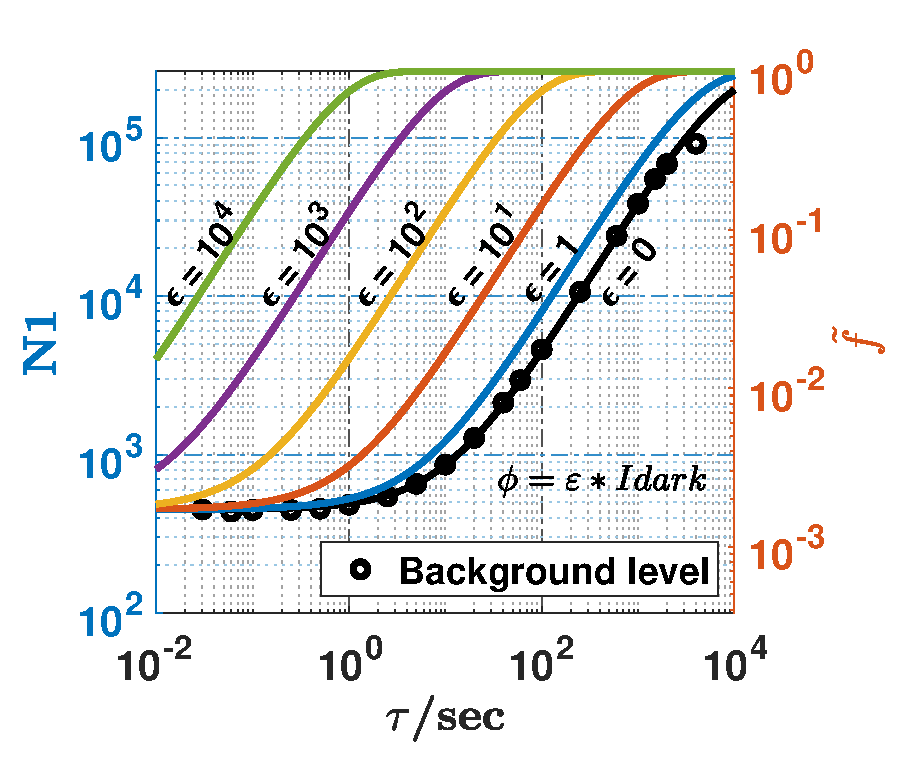
\includegraphics[width=0.4\linewidth]{fig3_model_fit/fig3A_fitmodel_ModelHeterogenN1Tau_dataTau.eps}\label{fig:SimuMeanVarN1:A}}  \qquad
\medskip
\subfloat[]{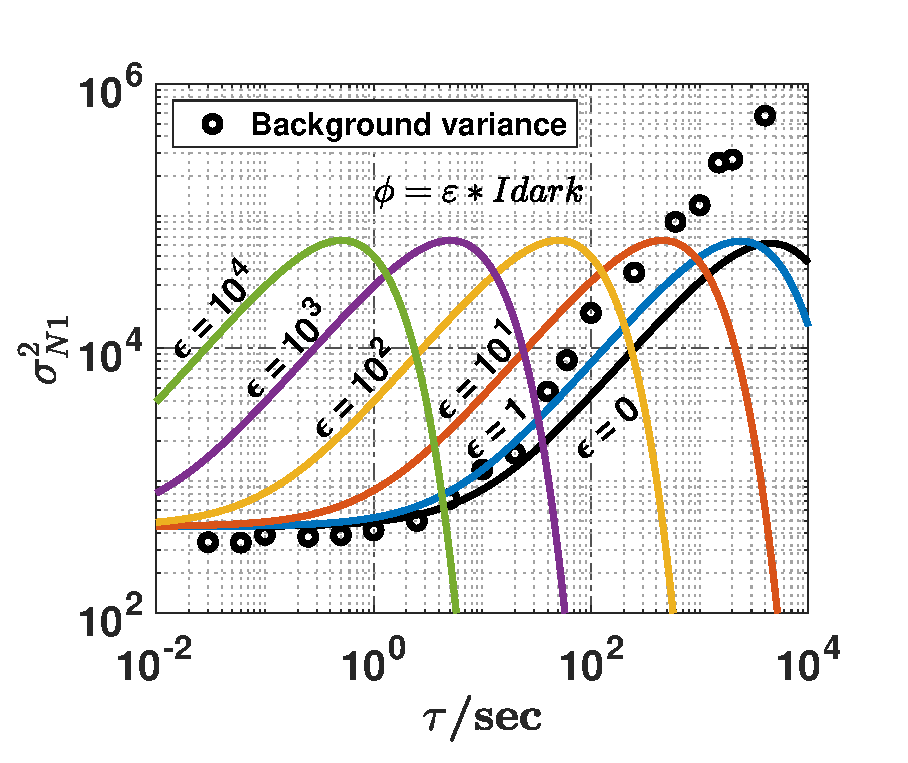
\includegraphics[width=0.4\linewidth]{fig3_model_fit/fig3B_fitmodel_ModelHeterogenVarN1Tau_TauData.eps}\label{fig:SimuMeanVarN1:B}} \qquad


\caption{{\bf wide detector response : simulation and data.}  The model  gives the simulation of the wide detector response N1 (N1 = $\sum_{ij}$pixels) \subref{fig:SimuMeanVarN1:A} and its variance  \subref{fig:SimuMeanVarN1:B} for different fluxes. The experimental noise (N1) and its variance are represented.}
\label{fig:SimuMeanVarN1}
\end{center}
\end{figure}
%%%%%%%%%%%%%%%%%%%


